\chapter{特征值与特征向量\ 矩阵标准形}

\section{Overview}
\begin{figure}[h]
	\centering
	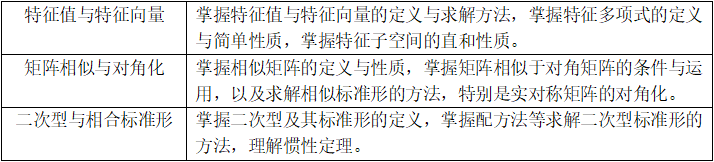
\includegraphics[scale=0.58]{9.png}
\end{figure}
注:由于本学期正交以及正定内容部分班级未讲授,因此也没有包含在本讲义中.讲义中可能有少量(2-3题)涉及
二次型正交标准化方法,可以简要了解或略过.
\section{特征值与特征向量}
从本章起,我们主要研究线性变换(而非一般线性映射)和方阵的性质.
\subsection{特征值与特征向量的定义与求解}
首先介绍线性变换和矩阵的特征值与特征向量的概念:
\begin{definition}
	设$\sigma$是线性空间$V(\mathbf{F})$上的一个线性变换,如果存在数$\lambda\in\mathbf{F}$
	和非零向量$\xi\in V$使得$\sigma(\xi)=\lambda\xi$,则称数$\lambda$为$\sigma$的一个特征值,
	并称非零向量$\xi$为$\sigma$属于其特征值$\lambda$的特征向量.
\end{definition}
必须注意特征向量为非零向量,否则零向量对任意$\lambda$都满足上面定义,从而失去“特征”的含义.
但是特征值可以为0,此时实际上就是线性变换的零空间.

特征值与特征向量的几何意义在于,某一线性变换的特征向量在经过变换后得到的向量与原先向量共线.

我们称关于同一个特征值$\lambda$的所有特征向量构成的集合记为$V_\lambda=\{\xi\ |\ \sigma(\xi)=\lambda\xi,\xi\in V\}$,
称为$\sigma$关于其特征值$\lambda$的特征子空间.
\begin{example}
	证明:$V_\lambda$是$V$的子空间.
\end{example}
实际上,$\sigma(\xi)=\lambda\xi$等价于$(\lambda I-\sigma)(\xi)=0$,故特征子空间就是线性变换
$\lambda I-\sigma$的核,核中必有非零向量(特征向量非零),故$\lambda I-\sigma$在$\lambda$为特征值时
必不满秩,故我们可以通过$|\lambda E-A|=0$求解特征值,其中$A$为$\sigma$在某组基下的矩阵.
对于特征向量的求解,求出$(\lambda E-A)X=0$的非零解就是特征向量在基下的坐标.

上面是线性变换的特征值与特征向量的定义,我们在考试中更一般地会遇到下述矩阵的特征值与特征向量的定义:
\begin{definition}
	设矩阵$A\in M_n(\mathbf{F})$,如果存在数$\lambda\in\mathbf{F}$和非零向量$X\in\mathbf{F}^n$使得
	$AX=\lambda X$,则称数$\lambda$为$A$的一个特征值,称非零向量$X$为$A$属于其特征值$\lambda$的特征向量.
\end{definition}
\begin{example}
	设$A=\begin{pmatrix}
		1 & -1 & 0 \\ 2 & 0 & 1 \\ 1 & a & 0
	\end{pmatrix}$,且存在非零向量$\alpha$使得$A\alpha=2\alpha$,求$\alpha$.
\end{example}
下面我们说明这两个定义的关系.实际上,假设$A$是$\sigma$在基$\alpha_1,\cdots,\alpha_n$下的表示矩阵,且
$\xi=(\alpha_1,\cdots,\alpha_n)X$,我们有
\begin{align*}
	\sigma(\xi)=\lambda\xi &\Leftrightarrow \sigma(\alpha_1,\cdots,\alpha_n)X=\lambda(\alpha_1,\cdots,\alpha_n)X \\
						   &\Leftrightarrow (\alpha_1,\cdots,\alpha_n)AX=(\alpha_1,\cdots,\alpha_n)(\lambda X) \\
						   &\Leftrightarrow AX=\lambda X
\end{align*}
因此$\lambda$同时是线性变换和矩阵的特征值,与基的选取无关,但$X$与基的选取有关.

我们在之前已经分析了求解特征值的方法,即求解$f(\lambda)=|\lambda E-A|$的根. 我们称其为矩阵$A$的特征多项式.
其$k$重根称为$k$重特征值(或称代数重数),对应的特征子空间维数称几何重数.

我们展开特征多项式得到以下定理:
\begin{theorem}
	对于$n$级矩阵$A=(a_{ij})$,记
	$$f(\lambda)=|\lambda E-A|=a_0\lambda^n+a_1\lambda^{n-1}+\cdots+a_{n-1}\lambda+a_n.$$
	则$a_0=1$,$a_n=(-1)^n|A|$,且$a_k$等于所有$k$级主子式之和乘以$(-1)^k$.
\end{theorem}
这一定理的证明无需掌握,并且关于特征多项式的进一步讨论也将在线性代数II中涉及.这里我们主要掌握两个特例,
即由韦达定理,我们有$\sum\limits_{i=1}^{n}\lambda_i=\sum\limits_{i=1}^{n}a_{ii}$,
$\prod\limits_{i=1}^{n}\lambda_i=|A|$,
即特征值按重数求和为矩阵的迹(即矩阵对角线元素之和),特征值按重数求积为矩阵行列式.
这一结论在解决某些问题时有一定作用.

\subsection{特征值的基本性质}
关于特征值,我们有如下基本性质,证明较为基本,可以自行完成:

设$\lambda$是线性空间$V(\mathbf{F})$上的线性变换$\sigma$的特征值,$\xi$是$\sigma$属于$\lambda$的特征向量,则

1. $k\lambda$是$k\sigma$的特征值,$\lambda^m$是$\sigma^m$的特征值,且$\xi$仍是相应特征向量.

2. 若$f(x)=a_nx^n+a_{n-1}x^{n-1}+\cdots+a_1x+a_0$是$\mathbf{F}$上的多项式,则$f(\sigma)(\xi)=f(\lambda)\xi$.

3. 设$\lambda$是$n$阶矩阵$A$的特征值,$A$可逆,则$\lambda^{-1}$是$A^{-1}$的特征值,$|A|\lambda^{-1}$是$A$的伴随矩阵
$A^*$的特征值,且特征向量不变.
\begin{example}
	回答以下问题:

	\textup{(1)}设$A$为三阶矩阵,$A^2-A-2E=O$,$|A|=2$,求$|A^*+3E|$\textup{;}
	
	\textup{(2)}设$A$为三阶矩阵,其特征值为$1$,$-2$,$-1$,求$|A|$,$A^*+3E$的特征值,$(A^{-1})^2+2E$的特征值
	以及$|A^2-A+E|$\textup{;}
	
	\textup{(3)}设$\alpha=(1,0,-1)^\mathrm{T}$,且$A=\alpha\alpha^\mathrm{T}$,求$|6E-A^n|$\textup{;}
	
	\textup{(4)}设$A$为三阶矩阵,其特征值为$-1$,$-1$,$5$,求$A_{11}+A_{22}+A_{33}$\textup{;}
	
	\textup{(5)}设$A$为三阶实对称矩阵,$A^2=A$且$r(A)=2$,求$|A+2E|$.
\end{example}

下面一个例子也是重要的结论,实际上在行列式专题已给出类似结论,但我们现在从特征值角度考虑这一结论:
\begin{example}
	回答以下两个问题:
	
	\textup{(1)}设$A,B$均为$n$阶矩阵,证明:$\lambda\neq 0$是$AB$的特征值,则$\lambda$也是$BA$的特征值\textup{;}
	
	\textup{(2)}设$A\in M_{m\times n}(\mathbf{C}),B\in M_{n\times m}(\mathbf{C})$,证明:
	$$\begin{pmatrix}
		AB & O \\ B & O
	\end{pmatrix}\sim\begin{pmatrix}
		O & O \\ B & BA
	\end{pmatrix},$$
	并由此推出$AB$和$BA$非零特征值相同,且$m=n$时有$|\lambda E-AB|=|\lambda E-BA|$.
\end{example}
不难发现(2)是(1)的推广.下面这一例子也是一些经典的结论,应当熟悉.
\begin{example}
	对下列矩阵$A$的特征值,能做出怎样的断言?
	
	\textup{(1)}$A$可逆/$A$不可逆/$E+A$可逆/$4E+A$不可逆\textup{;}
	
	\textup{(2)}$\det(E-A^2)=0$\textup{;}
	
	\textup{(3)}$AA^\mathrm{T}=A^\mathrm{T}A=E$(正交)/$A^2=E$(对合)/$A^2=A$(幂等)/$A^k=0$(幂零)\textup{;}
	
	\textup{(4)}$A=\lambda_0E+B$($\lambda_0$为常数,且已知$B$的$n$个特征值为$\lambda_1,\lambda_2,\cdots,\lambda_n$)\textup{;}
	
	\textup{(5)}$A$为对角块矩阵,即$A=\begin{pmatrix}
		A_1 &  &  &  \\  & A_2 &  &  \\  &  & \ddots &  \\  &  &  & A_m
	\end{pmatrix}$(与线代$\textup{II}$中不变子空间有关).
\end{example}
在上一小节我们讨论了特征值之和为迹的事实,实际上关于迹以及相关的幂零矩阵的讨论在专题三中已有涉及,
现在可以回过头去再看一些性质的证明.除此之外,我们还可以给幂零矩阵一个等价的定义:
\begin{theorem}
	一个方阵为幂零矩阵当且仅当其所有特征值均为$0$.
\end{theorem}
这一定理“仅当”部分证明比较基本,只需用到上述某一特征值性质即可,但“当”的部分无需掌握证明,需要用到线性代数II的
哈密顿-凯莱定理(事实上很多更进一步的讨论都要基于这一定理).
\subsection{特征向量的基本性质}
这一部分的定理与下一节中可对角化的等价条件直接相关,实际上有了本节的定理,可对角化条件是很显然的.
\begin{theorem}
	线性映射$\sigma$的不同特征值$\lambda_1,\cdots,\lambda_m$对应的特征向量$\xi_1,\cdots,\xi_m$线性无关.
\end{theorem}
\begin{theorem}
	线性映射$\sigma$的不同特征值$\lambda_1,\cdots,\lambda_m$对应的特征子空间$V_{\lambda_1},\cdots,V_{\lambda_m}$的和是直和,
	即$\dim(V_{\lambda_1}+V_{\lambda_2}+\cdots+V_{\lambda_m})=\sum_{j=1}^{m}\dim V_{\lambda_j}$.
\end{theorem}
以上两个定理的证明可以参考教材定理7.7及其推论,实际上二者等价,只需证出其中一个,另一个就是显然的.
两个定理有如下推论:

1. 若$\lambda_1,\cdots,\lambda_m$是线性映射$\sigma$互异的特征值,则$V_{\lambda_i}\cap\sum\limits_{j\neq i}V_{\lambda_j}=\{0\}
(i=1,\cdots,m)$,则一个特征向量不能属于多个特征值.这一推论来源于直和的一个等价条件,专题一的习题中有涉及.

2. $\sigma$的不同特征值$\lambda_1,\cdots,\lambda_m$对应的特征子空间$V_{\lambda_1},\cdots,V_{\lambda_m}$的基向量
合在一起构成的向量组线性无关,且是$V_{\lambda_1}+V_{\lambda_2}+\cdots+V_{\lambda_m}$的基.

接下来这个定理说明了代数重数和几何重数之间的关系:
\begin{theorem}
	$n$维线性空间$V(\mathbf{F})$的线性变换$\sigma$的每个特征值$\lambda_i$的重数(代数重数)大于等于其特征子空间$V_{\lambda_i}$的维数
	(几何重数).
\end{theorem}
这一定理的证明比较复杂,版本也很多,有兴趣的同学可以了解.
\subsection{习题}
\centerline{\heiti A组}
\begin{enumerate}
	\item 设$\sigma$是线性空间$\mathbf{R}[x]_3$上的线性变换,它在基$1,x,x^2$下的矩阵为
	$$A=\begin{pmatrix}
		1 & 2 & 2 \\ 2 & 1 & 2 \\ 2 & 2 & 1
	\end{pmatrix}.$$
	求$\sigma$的特征值与特征子空间.
	\item 设$A,P$都是3阶方阵,$P$可逆,已知$A$的特征值$\lambda_1=1,\lambda_2=-1,\lambda_3=2$,$B=A^3-5A^2$,
	求$|B|$,$|A+5E|$,$|5E+P^{-1}AP|$.
	\item 设$A=\begin{pmatrix}
		a & -1 & c \\ 5 & b & 3 \\ 1-c & 0 & -a
	\end{pmatrix}$,$|A|=-1$,$\alpha=(-1,-1,1)^\mathrm{T}$为$A^*$的特征向量,求$A^*$的特征值及$a,b,c$
	和$A$对应的特征值$\mu$.
	\item 设$A,B\in M_n(\mathbf{F})$,$AB=BA$,证明:若$X$是矩阵$A$属于特征值$\lambda_0$的特征向量,则
	$BX\in V_{\lambda_0}$(注:本题是解决很多$AB=BA$类问题的基础).
\end{enumerate}
\centerline{\heiti B组}
\begin{enumerate}
	\item 设$A,B$都是$n$阶矩阵,且$r(A)+r(B)<n$,证明:$A,B$有相同的特征值和特征向量.
	\item 设$V(\mathbf{F})$是$n$维线性空间,$\sigma\in L(V,V)$,证明:
	
	(1)若$\alpha,\beta$是$\sigma$的属于不同特征值的特征向量,则$c_1c_2\neq 0$时,$c_1\alpha+c_2\beta$
	不是$\sigma$的特征向量;

	(2)$V$中的每一非零向量都是$\sigma$的特征向量$\iff\sigma=c_0I_V$,其中$c_0\in\mathbf{F}$是一个常数,
	$I_V$是恒等变换.
	\item 设$A,B\in M_n(\mathbf{C})$,$B$的特征多项式$f(\lambda)=|\lambda E-B|$.证明:$f(A)$可逆的充要条件
	是$B$的任一特征值都不是$A$的特征值.
	\item 设$\lambda_1,\lambda_2,\cdots,\lambda_n$是矩阵$A=(a_{ij})_{n\times n}$的$n$个特征值,证明:
	$\lambda_1^2,\lambda_2^2,\cdots,\lambda_n^2$是$A^2$的$n$个特征值,且$\sum\limits_{i=1}^{n}\lambda_i^2=
	\sum\limits_{j=1}^{n}\sum\limits_{k=1}^{n}a_{jk}a_{kj}$.
	\item 设$A$为$n$阶矩阵,$X_1,X_2,X_3$为$n$元列向量,且$AX_1=kX_1(X_1\neq 0),AX_2=lX_1+kX_2,
	AX_3=lX_2+kX_3(l\neq 0)$,证明:$X_1,X_2,X_3$线性无关.
\end{enumerate}
\centerline{\heiti C组}
\begin{enumerate}
	\item 证明:若$AB=BA$,则$A$和$B$至少有一个共同的特征向量.
\end{enumerate}

\section{矩阵相似与对角化}
\subsection{矩阵相似的定义与性质}
我们早在线性映射矩阵表示专题中提到这一定理:
\begin{theorem}
	\textbf{基的选择对映射矩阵的影响}
	
	设线性变换$\sigma \in L(V,V)$,$B_1=\{\alpha_1,\dots,\alpha_n\}$和$B_2=\{\beta_1,\dots,\beta_n\}$
	是线性空间的$V(F)$的两组基,基$B_1$变为基$B_2$的变换矩阵为$C$,如果$\sigma$在基$B_1$下的矩阵为$A$,
	则$\sigma$关于基$B_2$所对应的矩阵为$C^{-1}AC$.
\end{theorem}
定理相关习题在相关章节有介绍,教材也有例题.这一定理研究同一个映射在不同基下表示矩阵之间的关系.
我们将具有如上性质的两个矩阵的关系称为相似的,规范定义如下:
\begin{definition}
	若对于$A,B\in M_n(\mathbf{F})$,存在可逆矩阵$C\in M_n(\mathbf{F})$, 使得
	$C^{-1}AC=B$,则称$A$相似于$B$,记作$A\sim B$.
\end{definition}
相似矩阵有以下基本性质,证明较为基本,请自行完成:

1. 相似是一种等价关系;两矩阵相似必相抵(秩相等);

2. $A\sim B$可以得到$A^\mathrm{T}\sim B^\mathrm{T}$,$A^m\sim B^m$,更一般地,对于任意多项式$f(x)$都有$f(A)\sim f(B)$,且
若$B=P^{-1}AP$,有$f(B)=P^{-1}f(A)P$.除此之外还有$A^*\sim B^*$,若$A,B$可逆,有$A^{-1}\sim B^{-1}$,$A^*\sim B^*$;

3. $A_1\sim B_1$,$A_2\sim B_2$不一定有$A_1+A_2\sim B_1+B_2$,只有当$P^{-1}A_1P=B_1,P^{-1}A_2P=B_2$时
(即相同的过渡矩阵$P$)才有$P^{-1}(A_1+A_2)P=B_1+B_2$;

4. 若$A_1\sim B_1$,$A_2\sim B_2$,则有
$$\begin{pmatrix}
	A_1 & O \\ O & A_2
\end{pmatrix}\sim\begin{pmatrix}
	B_1 & O \\ O & B_2
\end{pmatrix}\textup{;}$$

5. 相似矩阵有相同的特征多项式(逆命题不成立),即$A\sim B$有$|\lambda E-A|=|\lambda E-B|$,从而有相同的
迹,行列式,特征值,但特征向量不一定相同;

6. 与幂等矩阵相似的仍幂等,与对合矩阵相似的仍对合,与幂零矩阵相似的仍幂零
(但与正交矩阵相似的不一定正交,但与正交矩阵正交相似的是正交矩阵).
\begin{example}
	证明:两个可对角化的同阶矩阵特征值相同(包括重数)等价于它们相似.对于不可对角化的矩阵来说,这一结论还成立吗?
\end{example}
\begin{example}
	(教材定理$4.10$推广)设$P^{-1}AP=B$,证明:$A,B$分别属于同一特征值$\lambda$的特征向量$X$和$Y$满足$Y=P^{-1}X$.
\end{example}
一些题目可能需要判断矩阵是否相似,实际上我们有如下基本方法:
\begin{enumerate}
	\item 定义法:找到$P$使得$P^{-1}AP=B$即可,这一般是$A,B$没给出具体矩阵的做法,例如上面的性质证明;
	\item 我们也可以先计算两者特征多项式是否相等(即特征值是否一致),若不一致则一定不相似,得到结论,若一致且均为实对称矩阵则相似,
	否则不一定相似.于是对于这种特征值一致的情况,我们进行对角化,情况如下:
	\begin{enumerate}
		\item 若两矩阵均可对角化,则两矩阵相似(上述例题结论);
		\item 若一个矩阵可对角化,另一个矩阵不可对角化,则一定不相似;
		\item 若两个矩阵都不可对角化,不一定相似.需要两矩阵各个特征值的几何重数(即各个特征子空间维数)都一致才相似,否则不相似
		(了解结论即可,具体原因线性代数II会涉及).
	\end{enumerate}
\end{enumerate}
\begin{example}
	设$A,B\in M_n(\mathbf{F})$,证明:若$A$可逆,则$AB\sim BA$.
\end{example}
\begin{example}
	设$A=\begin{pmatrix}
		0 & 0 & 1 \\ 0 & 1 & 0 \\ 1 & 0 & 0
	\end{pmatrix},B=\begin{pmatrix}
		-1 & 0 & 0 \\ 0 & 0 & 1 \\ 0 & -1 & 2
	\end{pmatrix}$,判断$A$与$B$是否相似.
\end{example}
最后我们谈一个拓展内容,我们考虑矩阵方程$AX-XB=O$,若$A,B$都是$n$阶方阵且$X$可逆,则$A$与$B$相似,所以
这一矩阵方程的解空间的维数实际上刻画了$A$与$B$的相似程度.我们有如下结论,不要求掌握,也不要求证明,了解即可:
\begin{theorem}
	设$A,B$分别为数域$P$上$n$阶、$m$阶方阵,则$A,B$有$r$个两两不等的公共特征值,则矩阵方程$AX-XB=O$有秩为
	$r$的矩阵解.反之,若数域为复数域,矩阵方程$AX-XB=O$有秩为$r$的矩阵解,则$A,B$至少有$r$个公共的特征值
	(计重数).
\end{theorem}
由此,复数域上$n$阶、$m$阶方阵$A,B$的矩阵方程$AX=XB$只有零解的充要条件是$A,B$没有公共特征值.
\subsection{可对角化的条件}
我们知道,矩阵可对角化意味着矩阵相似于一个对角矩阵,即存在可逆矩阵$P$使得$P^{-1}AP=\Lambda$,其中
$\Lambda=\textup{diag}(\lambda_1,\lambda_2,\cdots,\lambda_n)$为对角矩阵.

将$P^{-1}AP=\Lambda$变形为$AP=P\Lambda$,并将矩阵$P$按列分块为$P=(X_1,X_2,\cdots,X_n)$,则有
$A(X_1,X_2,\cdots,X_n)=(X_1,X_2,\cdots,X_n)\textup{diag}(\lambda_1,\lambda_2,\cdots,\lambda_n)$,
利用分块矩阵乘法我们有$AX_j=\lambda_jX_j(X_j\neq 0,j=1,2,\cdots,n)$.

通过上述过程我们容易证明$n$维空间上线性映射可对角化当且仅当有$n$个线性无关的特征向量.并且这一过程也是我们
求解对角化问题的基本方法.综合上述推导以及上一节中2.3小节的定理,我们有如下结论:
\begin{theorem}
	设$V$是数域$\mathbf{F}$上的$n$维线性空间,$\sigma$是$V$上的线性变换,$\lambda_1,\lambda_2,\cdots,\lambda_s\in\mathbf{F}$
	是$\sigma$的所有互异特征值,则以下条件等价:
	
	\textup{(1)}$\sigma$可对角化\textup{;}
	
	\textup{(2)}$\sigma$有$n$个线性无关的特征向量,它们构成$V$的一组基\textup{;}
	
	\textup{(3)}$V=V_{\lambda_1}\oplus V_{\lambda_2}\oplus\cdots\oplus V_{\lambda_s}$\textup{;}
	
	\textup{(4)}$n=\dim V_{\lambda_1}+\dim V_{\lambda_2}+\cdots+\dim V_{\lambda_s}$\textup{;}
	
	\textup{(5)}$\sigma$每个特征值的代数重数等于几何重数\textup{.}
\end{theorem}
实际上对于矩阵我们有对应的定理,此处不再赘述.我们有一个推论,若有$n$个互不相同的特征值则一定能对角化,
这是(2)的直接推论,但反之不成立,有多重特征值的矩阵也可能可以对角化,只要满足上述条件.

实际上由特征值的性质,我们容易知道数域$\mathbf{F}$上矩阵$A$可对角化,则$A^*$可对角化,对于数域$\mathbf{F}$上
任意多项式$f(x)$,$f(A)$也可对角化,且$A$可逆时,$A^{-1}$也可对角化.
\begin{example}
	证明$r$阶上三角矩阵$(r>1)$
	$$J_0=\begin{pmatrix}
		\lambda_0 & 1 &  &  \\ 
		  & \lambda_0 & \ddots &  \\
		  &  & \ddots &  1 \\
		  &  &  &  \lambda_0
	\end{pmatrix}$$
	不与对角阵相似.
\end{example}
\begin{example}
	设$A=(a_{ij})_{n\times n}$是上三角矩阵.
	
	\textup{(1)}求$A$的全部特征值\textup{;}

	\textup{(2)}若$A$主对角元互不相等,证明:$A$与对角阵相似\textup{;}

	\textup{(3)}若$n$个主对角元相等且$A$不为对角矩阵,证明:$A$不与对角阵相似.
\end{example}
\begin{example}
	设$\alpha$和$\beta$是$\mathbf{R}^n(n>1)$中两个列向量,$A=\alpha\beta^\mathrm{T}\neq O$.
	
	\textup{(1)}求$A$的特征值\textup{;}
	
	\textup{(2)}证明:$\alpha^\mathrm{T}\beta=0\iff A$不可对角化.
\end{example}
最后需要说明一点,如果一个矩阵可对角化,那么我们可以将其表示为$A=P\Lambda P^{-1}$,其中
$P$可逆(即所谓特征值分解).实际上相抵、相合都有类似的表示思想,在解决一些题目时是重要的.
\begin{example}
	设$n$阶实对称矩阵$A$的特征值$\lambda_i\ge 0(i=1,\cdots,n)$.证明:存在特征值都是非负数的实对称矩阵
	$B$使得$A=B^2$(本题可推广为多次幂).
\end{example}
\begin{example}
	设三阶矩阵$A$的特征值为$\lambda_1=-2,\lambda_2=1,\lambda_3=2$,对应的特征向量分别为
	$\alpha_1=(1,1,0)^\mathrm{T},\alpha_2=(1,0,1)^\mathrm{T},\alpha_3=(1,1,1)^\mathrm{T}$,求矩阵$A$.
\end{example}
\subsection{对角化问题的一般解法}
下面我们总结一下求解对角化问题的基本方法:对于一个$n$阶可对角化矩阵$A$,求变换矩阵$P$使得$P^{-1}AP=\Lambda$,步骤如下:

1. 求出$A$的所有不同特征值;

2. 求出$A$在不同特征值下的特征子空间的基;

3. 将这组基按列排列成矩阵$P$.

这一过程的合理性在本小节开头就有叙述.下面我们来看一个基本的例子:
\begin{example}
	设$A=\begin{pmatrix}
		2 & 2 & 0 \\ 8 & 2 & a \\ 0 & 0 & 6
	\end{pmatrix}$相似于对角矩阵,求常数$a$,并求可逆矩阵$P$使得$P^{-1}AP$为对角矩阵.
\end{example}
除此之外,我们还可以利用对角化求解矩阵的幂的问题,在专题三中已经介绍,此处不再赘述.

\subsection{实对称矩阵对角化}
这一部分内容因为涉及正交的概念所以有班级未提及,因此我们只能回顾不涉及正交的部分.
教材定义7.7给出了共轭矩阵的概念,下方给出了大量的性质,此处不再赘述.我们的重点在于以下两个定理:
\begin{theorem}
	实对称矩阵的特征值都是实数.
\end{theorem}
这一定理的证明应当掌握,特别是如何证明实数的方法(即共轭等于自身).
\begin{theorem}
	实对称矩阵一定可以相似对角化.
\end{theorem}
这一定理证明只需要讲教材定理7.13除去正交即可.以上两个定理十分重要,是我们接下来讨论以及解决一些问题的基础.
\begin{example}
	已知$A$是实反对称矩阵,证明:

	\textup{(1)}$A$的特征值必为$0$或纯虚数\textup{;}

	\textup{(2)}$E-A^2$是可逆矩阵.
\end{example}
当然要注意的一点是,因为无法涉及正交的内容,本节习题中所有的对角化问题都无需进行施密特正交化,只需要像
上一小节介绍的方法那样求出一般的可逆矩阵即可.
\subsection{幂等矩阵}
若$n$阶方阵$A$满足$A^2=A$,则$A$称为幂等矩阵.幂等矩阵具有如下基本性质,请自行证明:

1. $A$是幂等矩阵等价于$r(A)+r(A-E)=n$;

2. $A$为幂等矩阵则一定可对角化,特征值为0和1,其中1的重数等于$r(A)$;

3. $A$是幂等矩阵时,$r(A)=\textup{tr}(A)$;

4. 所有秩为1迹也为1的矩阵均为幂等矩阵.

实际上,幂等矩阵还有很多其他的性质,我们可以回到映射的角度去理解这一矩阵,
例如其与投影变换的等价性(与像空间、核空间有关,可以自行证明).
\begin{example}
	设$A$,$B$为两个$n$阶幂等矩阵,证明:

	\textup{(1)}$A+B$为幂等矩阵当且仅当$AB=BA=O$;

	\textup{(2)}$A-B$为幂等矩阵当且仅当$AB=BA=B$;

	\textup{(3)}若$AB=BA$,则$AB$为幂等矩阵,反之,若$AB$为幂等矩阵,是否必有$AB=BA$;

	\textup{(4)}若$E-A-B$可逆,则$r(A)=r(B)$.
\end{example}
\subsection{习题}
注:这一专题的很多习题需要大家熟练掌握所学的性质,例如熟练掌握可对角化的充要条件,对于题目给出的“实对称”或者
特征值、特征向量个数等关键词以及一些基本题型等保持敏感,并合理运用,需要各位同学自己多多熟悉(当然最终考试
难度可能略低于这些问题).除此之外,在考试判断题中也可能有一些基本性质的考察,因为本章涉及性质很多,请千万
不要混淆滥用,应当学会证明和给反例,而非死记硬背.

\centerline{\heiti A组}
\begin{enumerate}
	\item 求矩阵

	$$
	A=\left(\begin{array}{ccc}
	0 & -1 & 1 \\
	-1 & 0 & 1 \\
	1 & 1 & 0
	\end{array}\right)
	$$
	
	的所有特征值,对应的特征子空间,以及与 $A$ 相似的一个对角矩阵.
	\item 设$A=\begin{pmatrix}
		a & b \\ c & d
	\end{pmatrix}$为二阶实矩阵.

	(1)若$|A|<0$,问:$A$与对角矩阵是否相似;

	(2)若$ad-bc=1$,$|a+d|>2$,问:$A$是否可对角化.
	\item 设$A=\begin{pmatrix}
		1 & 1 & a \\ 1 & a & 1 \\ a & 1 & 1
	\end{pmatrix}$,$\beta=\begin{pmatrix}
		1 \\ 1 \\ -2
	\end{pmatrix}$,方程组$AX=\beta$有解但不唯一.

	(1)求$a$的值;

	(2)求可逆矩阵$P$使得$P^{-1}AP$为对角矩阵.
	\item 设$A$为三阶矩阵,$\alpha_1,\alpha_2,\alpha_3$线性无关,且
	$A\alpha_1=\alpha_1,A\alpha_2=\alpha_1+\alpha_2-2\alpha_3,A\alpha_3
	=\alpha_1-2\alpha_2+\alpha_3$,求$A$的特征值.
	\item 设三阶实对称矩阵$A$的各行元素之和为3,向量$\alpha_1=(-1,2,-1)^\mathrm{T}$,$\alpha_2=(0,-1,1)^\mathrm{T}$
	是方程组$AX=0$的两个解,求矩阵$P$使得$P^{-1}AP$为对角矩阵.
	\item 解决以下关于可对角化的基本问题:
	
	(1)设$A$为$n$阶矩阵,且$A^2=2A$,证明:$A$可对角化;

	(2)设$a\neq b$,且$(aE-A)(bE-A)=O$,证明:$A$可对角化(特例:对合矩阵);

	(3)设$A$为$n$阶非零矩阵,且$A^m=O(m\in\mathbf{N^+},m>1)$,
	证明:$A$不可对角化;

	(4)秩为1的矩阵$A$可对角化的充要条件是$A$的迹不为0;

	(5)设$A$为二阶矩阵,非零向量$\alpha$不是$A$的特征向量,且$A^2\alpha-
	3A\alpha+2\alpha=0$,证明:$\alpha$和$A\alpha$线性无关且$A$可对角化并求
	与$A$相似的对角矩阵.
\end{enumerate}
\centerline{\heiti B组}
\begin{enumerate}
	\item 已知$\mathbf{R}^3$的一个线性变换
	$$\sigma(x_1,x_2,x_3)=(2x_1-2x_2,-2x_1+x_2-2x_3,-2x_2).$$
	(1)求$\sigma$关于自然基$\{e_1,e_2,e_3\}$所对应的矩阵$A$;
	
	(2)求$\sigma$关于基$\{(1,1,1),(0,1,1),(0,0,1)\}$所对应的矩阵$B$;

	(3)求矩阵$C_1$,使$C_1^{-1}BC_1=A$.
	\item 设$A=\begin{pmatrix}
		0 & 0 & 1 \\ 0 & 0 & 0 \\ 1 & 0 & 0
	\end{pmatrix},B=\begin{pmatrix}
		1 & 0 & 0 \\ 0 & 1 & 2 \\ 0 & -1 & -2
	\end{pmatrix}$,证明:$A\sim B$,并求可逆矩阵$P$使得$P^{-1}AP=B$.
	\item 已知$A=\begin{pmatrix}
		2 & 0 & 0 \\ 0 & 0 & 1 \\ 0 & 1 & x
	\end{pmatrix}$与$B=\begin{pmatrix}
		2 & 0 & 0 \\ 0 & y & 0 \\ 0 & 0 & -1
	\end{pmatrix}$相似.

	(1)求$x$和$y$;

	(2)求一个可逆矩阵$P$,使$P^{-1}AP$为对角矩阵.
	\item 设$A=\begin{pmatrix}
		1 & 2 & 0 & 0 & 0 \\ 4 & 3 & 0 & 0 & 0 \\ 0 & 0 & 1 & -3 & 3 \\ 0 & 0 & 3 & -5 & 3 \\ 
		0 & 0 & 6 & -6 & 4
	\end{pmatrix}$,求$A$的特征值.若$A$可对角化,求可逆矩阵$P$,使$P^{-1}AP$为对角矩阵.
	\item 设三阶矩阵$A$的特征值为$\lambda_1=1,\lambda_2=2,\lambda_3=3$,它们对应的特征向量为$\xi_1=(1,1,1)^\mathrm{T},
	\xi_2=(1,2,4)^\mathrm{T},\xi_3=(1,3,9)^\mathrm{T}$,又$\beta=(1,1,3)^\mathrm{T}$,计算$A^n\beta$.
	\item 设$A=\begin{pmatrix}
		3 & 4 & 0 & 0 \\ 4 & -3 & 0 & 0 \\ 0 & 0 & 2 & 4 \\ 0 & 0 & 0 & 2
	\end{pmatrix}$,求$A^n(n\in\mathbf{N^*})$.
	\item 设$A$为$n$阶实对称幂等矩阵,$r(A)=r$,求$|A-2E|$.
	\item 已知三阶矩阵$A$和三元列向量$X$,使得向量组$X,AX,A^2X$线性无关,且满足
	$$A^3X=3AX-2A^2X.$$

	(1)记$P=(X\ AX\ A^2X)$,求三阶矩阵$B$使得$A=PBP^{-1}$;

	(2)计算行列式$|A+E|$.
	\item (秩为1的矩阵)设$n$阶矩阵$A$的元素均为1.
	
	(1)求$A$的特征值,并求矩阵$P$使得$P^{-1}AP$为对角矩阵;

	(2)若$f(x)$是$x$的$m$次多项式,且常数项为0,证明:存在$k\in\mathbf{R}$使得$f(A)=kA$,并求出$k$;

	(3)设$B$是$n$阶实对称矩阵,每行元素之和都为$b$,若$b$是$f(\lambda)=|\lambda E-B|$的单根,求$B$属于$b$的特征向量;
	当$f(\lambda)=(\lambda-b)g(\lambda)$时(其中$f(B)=0$),证明:$g(B)=kA$,其中$k$为常数,
	$A$为元素全部为1的$n$阶矩阵.
	\item 设$A,B\in M_n(\mathbf{F})$,$A$有$n$个不同的特征值,证明:$AB=BA$当且仅当$A$的特征向量也是$B$的特征向量
	(推论:若$A,B$均可对角化,$AB=BA$,则对角化的过渡矩阵可以相同).
\end{enumerate}
\centerline{\heiti C组}
\begin{enumerate}
	\item 设$B=\alpha\alpha^\mathrm{T}$,其中$\alpha=(a_1,\cdots,a_n)^\mathrm{T}\neq 0(a_i\in\mathbf{R},i=1,2,\cdots,n)$.
	
	(1)证明:$B^k=tB$,其中$k$为正整数,$t$为常数,并求$t$;

	(2)求可逆阵$P$使得$P^{-1}BP$为对角矩阵,并写出该对角矩阵.
	\item 设$A$相似于对角矩阵,$\lambda_0$是$A$的特征值,$X_0$是$A$对应于$\lambda_0$的特征向量,证明:
	
	(1)$r(A-\lambda_0 E)^2=r(A-\lambda_0 E)$;

	(2)不存在$Y$使得$(A-\lambda_0 E)Y=X_0$.
	\item 设$A,B$为$n$阶矩阵,且$A+B=AB$,求证:
	
	(1)$A,B$的特征向量是公共的;

	(2)$A$相似于对角矩阵当且仅当$B$相似于对角矩阵;

	(3)$r(A)=r(B)$.
	\item 设$A,B\in M_n(\mathbf{R})$,证明$A$与$B$在$\mathbf{R}$上相似当且仅当在
	$\mathbf{C}$上相似.

	注:实际上相似这一性质与数域无关,本题是这一结论的特例.
	\item (数学归纳法)证明:对任一$n$阶矩阵$A\in M_n(\mathbf{C})$,存在可逆矩阵$P$使得$P^{-1}AP$
	为上三角矩阵.
	\item 设$A,B\in M_n(\mathbf{F})$,$A$有$n$个不同的特征值,且$AB=BA$,证明:存在次数小于等于$n-1$
	的多项式$f(x)$使得$B=f(A)$.
\end{enumerate}

\section{二次型及其标准形}
\subsection{二次型的定义}
\begin{definition}
	$n$个元$x_1,x_2,\cdots,x_n$的二次齐次多项式
	\begin{align*}
		f(x_1,x_2,\cdots,x_n) &= \sum_{i=1}^{n}a_{ii}x_i^2+\sum\limits_{1\le i<j\le n}2a_{ij}x_ix_j \\
							  &= a_{11}x_1^2+a_{22}x_2^2+\cdots+a_{nn}x_n^2 \\
							  &\ \ \ +2a_{12}x_1x_2+\cdots+2a_{1n}x_1x_n+2a_{23}x_2x_3+\cdots+2a_{n-1,n}x_{n-1}x_n
	\end{align*}
	称为数域$\mathbf{F}$上的$n$元二次型(简称二次型).
\end{definition}
本学期研究的主要是实二次型.若令$a_{ij}=a_{ji}(1\le i<j\le n)$,则二次型可表示为
$$f(x_1,x_2,\cdots,x_n)=\sum_{i=1}^{n}\sum_{j=1}^{n}a_{ij}x_ix_j=X^\mathrm{T}AX$$
其中$X=(x_1,x_2,\cdots,x_n)^\mathrm{T}\in\mathbf{R}^n$,$A=(a_{ij})_{n\times n}$为实对称矩阵,
并称对称矩阵$A$为二次型$f(x_1,x_2,\cdots,x_n)$的矩阵.

注意,二次型实际上是一个$\mathbf{R}^n\to\mathbf{R}$的函数,所以本质上代入$x_1,\cdots,x_n$后就是一个实数,写成矩阵形式
我们也可以发现矩阵相乘结果为$1\times 1$矩阵,即一个实数,因此不必把二次型想得过于复杂.

同时需要注意,二次型对应矩阵一定是对称矩阵.实际上一个形如$f(x_1,x_2,\cdots,x_n)=\sum\limits_{i=1}^{n}\sum\limits_{j=1}^{n}a_{ij}x_ix_j$
的函数可以对应的矩阵是很多的,但我们要求$a_{ij}=a_{ji}$才能得到二次型对应的矩阵.
\begin{example}
	已知二次型
	$$f(X)=(x_1,x_2,x_3,x_4)\begin{pmatrix}
		1 & 2 & 3 & -4 \\ 3 & 2 & 1 & 4 \\ -4 & 3 & -7 & 2 \\ 0 & -6 & 8 & 4
	\end{pmatrix}\begin{pmatrix}
		x_1 \\ x_2 \\ x_3 \\ x_4
	\end{pmatrix}.$$
	写出二次型$f(X)$的矩阵.
\end{example}
\begin{example}
	回答以下问题:

	\textup{(1)}已知$A$是一个$n$阶矩阵,则$A$为反对称矩阵的充要条件是对任意$n$元列向量$X$都有$X^\mathrm{T}AX=0$\textup{;}
	
	\textup{(2)}若二次型$f(x_1,x_2,\cdots,x_n)=X^\mathrm{T}AX$对任意$n$元列向量$X$都有$f(x_1,x_2,\cdots,x_n)=0$,证明:$A=O$\textup{;}
	
	\textup{(3)}设二次型$f(x_1,x_2,\cdots,x_n)=X^\mathrm{T}AX$,$g(x_1,x_2,\cdots,x_n)=X^\mathrm{T}BX$,证明:若$f(x_1,x_2,\cdots,x_n)=
	g(x_1,x_2,\cdots,x_n)$,则$A=B$.
\end{example}
\subsection{矩阵相合的定义与性质}
\begin{definition}
	我们称$n$阶矩阵$A$相合于$B$(记作$A\simeq B$),如果存在可逆矩阵$C$使得$B=C^\mathrm{T}AC$.
\end{definition}
矩阵相合(合同)有如下基本性质:

1. 合同是等价关系;合同不同于相似,是与数域有关的;合同要求$C$必须可逆,因此是一种特殊的相抵;

2. $A\simeq B$一般不能得到$A^m\simeq B^m$(但是$A,B$为实对称矩阵时可以),但如果可逆,我们有
$A^{-1}\simeq B^{-1}$,同时如果$A_1\simeq A_2,B_1\simeq B_2$,则有$\begin{pmatrix}
	A_1 & O \\ O & B_1
\end{pmatrix}\simeq\begin{pmatrix}
	A_2 & O \\ O & B_2
\end{pmatrix}$;

3. $A\simeq B$表明$A$可以每次做相同的初等行列变换得到$B$,反之亦然.这实际上就是初等变换法求相合标准形
的基本原理,详见教材260页小字部分,感兴趣同学可以了解,一般不会要求使用这一方法.

\begin{example}
	设$A\simeq B$,$C\simeq D$,且它们都是$n$阶实对称矩阵,问:$A+C\simeq B+D$成立吗?
\end{example}
\begin{example}
	判断:矩阵相似是否一定合同?矩阵合同是否一定相似?对于实对称矩阵上述论断又是否正确呢?
	正确请说明理由,不正确请举出反例.
\end{example}
实际上,教材中引入合同与二次型使用了双线性函数这一概念,实际上与双线性函数的度量矩阵有关,感兴趣的同学可以了解,
但这部分属于小字,考试一般不做考查要求.
\subsection{二次型标准形的定义与求解}
实际上二次型可以视为一个空间曲线/曲面方程,我们希望这些方程化为标准形式,有助于我们讨论一些问题.
由于实二次型对应矩阵为实对称矩阵,实对称矩阵一定可以相似对角化,故有下面的定理:
\begin{theorem}
	任意二次型$f(X)=X^\mathrm{T}AX$总可以通过可逆的线性变换$X=PY$(其中$P$可逆)化为标准形,
	即$f(X)=X^\mathrm{T}AX\xlongequal{X=PY}Y^\mathrm{T}(P^\mathrm{T}AP)Y=d_1y_1^2+d_2y_2^2+\cdots+d_ny_n^2$.
\end{theorem}
一般而言,我们有三种方法求解二次型标准形,分别为正交变换法,配方法和初等变换法.正交变换法由于涉及正交因此不作要求,
初等变换法之前已经提及并且较为复杂,不推荐优先使用.因此我们接下来主要使用配方法.

注意,求二次型标准形不应使用之前求相似标准形的一般方法,因为只有正交矩阵才能保证$P^{-1}=P^\mathrm{T}$,一般矩阵无法保证.
当然实际上求得的对角矩阵都是由特征值按重数排列而成的,只是矩阵$P$不合要求,应当做施密特正交化.

配方法的思想非常简单,就是利用配方消除混合乘积项,将二次型表示成几个平方和的形式,最后通过坐标变换$X=CY$(又称仿射变换,其中$C$可逆)
化标准形.
\begin{example}
	用配方法把三元二次型
	$$f(x_1,x_2,x_3)=2x_1^2+3x_2^2+x_3^2+4x_1x_2-4x_1x_3-8x_2x_3$$
	化为标准形,并求所用的坐标变换$X=CY$即变换矩阵$C$.
\end{example}
配方法是合理的,因为$X=CY$,其中$C$可逆,则$X^\mathrm{T}AX=Y^\mathrm{T}(C^\mathrm{T}AC)Y$,配方法使得$C^\mathrm{T}AC$
为对角矩阵,因此可以得到相合标准形.但是这种方法不能用来求相似对角化,原因仍然是$C^{-1}=C^\mathrm{T}$需要$C$为正交矩阵,但
坐标变换矩阵不一定满足.所以一定要区分好求解相似、相合标准形使用的方法,不能因为题目经常给的是实对称矩阵而混淆,只有正交变换法
是通用的,因为正交矩阵满足$P^{-1}=P^\mathrm{T}$使得相似、相合的定义统一.

注意:有的同学可能知道正交变换法的具体操作流程,如果能保证计算正确且题目不强制配方法时可以使用,但是历年考试经常出现部分题目
求解特征值时三次方程解不出的情况,此时一定要立刻醒悟,转向配方法解决问题.

\subsection{相合规范形\ 惯性定理}
事实上,一个二次型通过正交变换标准化得到的对角矩阵对角线上元素为特征值按重数排列的结果,但是使用配方法、初等变换法则不一定,
甚至配方方式或者初等变换顺序不同都会产生不同的对角矩阵,因此相合标准形不唯一.但我们知道,相抵标准形唯一,相似标准形不考虑
排列组合因素也是唯一的,因此我们也需要统一相合标准形.

我们不难发现,任一对角矩阵一定相合于$\textup{diag}(1,\cdots,1,-1,\cdots,-1,0,\cdots,0)$(我们很容易写出对应的可逆变换矩阵),
我们称这一相合标准形为相合规范形,其中+1的个数称为矩阵的正惯性指数,-1的个数称为矩阵的负惯性指数.并且由于变换矩阵可逆,根据
相抵标准形的结论,我们有原矩阵$A$的秩$r(A)$等于这一对角矩阵的秩,于是也等于正负惯性指数之和.显然,$A$可逆时,其相合规范形
主对角元没有0.

但我们没有说明一个矩阵的相合规范形是否唯一,实际上这就是下面惯性定理的结果:
\begin{theorem}
	实对称矩阵的相合规范形唯一.
\end{theorem}
这一定理有很多等价表述,例如实对称矩阵正、负惯性指数唯一,或者实对称矩阵相合标准形中对角线上正、负、零的个数唯一.
或者实对称矩阵特征值中正、负、零的个数唯一等.
这一定理的证明方法比较经典,最关键的一步在于代入数值导出矛盾,代入的方法是在两种表达的正负号分界线前后分别置0,使得
两种表达形式一个大于0,一个小于等于0.
\begin{example}
	解答如下问题:

	\textup{(1)}设$n$元二次型$f(x_1,x_2,\cdots,x_n)=l_1^2+\cdots+l_p^2-l_{p+1}^2-\cdots-l_{p+q}^2$,其中$l_i(i=1,2,\cdots,p+q)$
	是关于$x_1,x_2,\cdots,x_n$的一次齐次式,证明:$f(x_1,x_2,\cdots,x_n)$的正惯性指数$\le p$,负惯性指数$\le q$\textup{;}
	
	\textup{(2)}已知$A$为$m$阶实对称矩阵,$C$为$m\times n$实矩阵,证明:$C^\mathrm{T}AC$的正负惯性指数
	分别小于等于$A$的正负惯性指数.
\end{example}
\begin{example}
	确定二次型$f(x_1,x_2,\cdots,x_{10})=x_1x_2+x_3x_4+x_5x_6+x_7x_8+x_9x_{10}$的秩以及正、负惯性指数.
\end{example}
惯性定理的“惯性”二字与物理中的惯性有关,实际上透露着某种不变性,根据惯性定理,我们有如下结论:

1. 我们可以按相合关系对全体$n$阶实对称矩阵分类,因为实对称矩阵相合意味着规范形唯一,我们可以按照+1、-1、0个数的不同
划分为$\cfrac{(n+1)(n+2)}{2}$个等价类(相抵、相似也是等价关系,可以思考划分等价类的方式与个数);

2. 实数域上两个实对称矩阵相合的充要条件是它们有相同的正负惯性指数,两个对角矩阵相合的充要条件是对角线上正、负、零个数相同.

注:复数域上两个对称矩阵相合的充要条件是它们的秩相同(可以思考其证明),例如$E_n$和$-E_n$在复数域上相合,但实数域上不相合.
\begin{example}
	设$A=\begin{pmatrix}
		1 & 2 & 0 \\ 2 & 1 & 0 \\ 0 & 0 & 3
	\end{pmatrix}$,$B=\begin{pmatrix}
		-2 & 0 & 0 \\ 0 & 2 & 1 \\ 0 & 1 & 2
	\end{pmatrix}$,判断$A$与$B$是否相合.
\end{example}
\subsection{标准形的应用}
我们在本学期讨论了三种标准形,即相抵标准形,相似标准形和相合标准形,实际上它们之间的关系我们已经讨论,
即相似一定相抵,相合一定相抵,但相似和相合互相没有包含关系.本节我们考虑一些基于矩阵分解的问题,利用之前所学的
相抵标准形、相似标准形、相合标准形的分解解决一些问题.本节内容可以选择性掌握.

首先看一个关于幂等矩阵的例题,需要用到相抵标准形、相似标准形的分解:
\begin{example}
	解答以下两个问题:

	\textup{(1)}证明:任意一个方阵都可以分解成一个可逆矩阵和一个幂等矩阵的乘积\textup{;}
	
	\textup{(2)}已知$A$是一个秩为$r$的$n$级非零矩阵,证明:$A$为幂等矩阵的充要条件是存在列满秩的$n\times r$矩阵$B$和行满秩的
	$r\times n$矩阵$C$使得$A=BC$且$CB=E_r$.
\end{example}
下面是一个利用相合标准形进行分解的例子:
\begin{example}
	(与正交有关)证明:每个秩为$r$的$n(r<n)$阶实对称矩阵均可表示为$n-r$个秩为$n-1$的实对称矩阵的乘积.
\end{example}
\subsection{习题}
\centerline{\heiti A组}
\begin{enumerate}
	\item 已知$A=\begin{pmatrix}
		2 & 2 & -2 \\ 2 & 5 & -4 \\ -2 & -4 & 4
	\end{pmatrix}$,分别用配方法和初等变换法将二次型$X^\mathrm{T}AX$化为标准形,并给出$X=CY$的变换矩阵$C$.
	\item 证明:秩为$r$的$n$阶实对称矩阵$A$可以表示为$r$个秩为1的实对称矩阵的和.
\end{enumerate}
\centerline{\heiti B组}
\begin{enumerate}
	\item 已知三元二次型$f(x_1,x_2,x_3)=2x_1x_2-2x_1x_3+2x_2x_3$.
	
	(1)利用配方法求其标准形,并写出坐标变换矩阵;
	
	(2)(与正交有关)求在$X=(x_1,x_2,x_3)^\mathrm{T}$满足条件$X^\mathrm{T}X=x_1^2+x_2^2+x_3^2=1$时的最小值.
	\item 设$A$为$n$阶实对称矩阵,$r(A)=n$,$A_{ij}$是$A=(a_{ij})_{n\times n}$中元素$a_{ij}$的代数余子式,
	二次型$f(x_1,x_2,\cdots,x_n)=\sum\limits_{i=1}^{n}\sum\limits_{j=1}^{n}\cfrac{A_{ij}}{|A|}x_ix_j$.

	(1)记$X=(x_1,x_2,\cdots,x_n)$,把$f(x_1,x_2,\cdots,x_n)$写成矩阵形式,并证明二次型$f(X)$的矩阵是$A^{-1}$;

	(2)二次型$g(X)=X^\mathrm{T}AX$与$f(X)$的规范形是否相同?说明理由.
	\item 设$f(x_1,x_2,x_3)=(x_1-x_3)^2+(x_2+ax_3)^2+(x_1+x_2)^2$.
	
	(1)就$a$的不同取值,求$f(x_1,x_2,x_3)=0$时的$X$;

	(2)求$f(x_1,x_2,x_3)$的规范形.
	\item 已知二次型$f(x_1,x_2,x_3)=(1-a)x_1^2+(1-a)x_2^2+2x_3^2+2(1+a)x_1x_2$的秩为2.
	
	(1)求常数$a$;

	(2)写出二次型$f(x_1,x_2,x_3)$规范形;

	(3)求方程$f(x_1,x_2,x_3)=0$的解.
	\item 设实二次型 $f(x_1,\ x_2,\ x_3)=ax_1^2+2x_2^2-2x_3^2+2bx_1x_3(b > 0)$,二次型对应的矩阵 $A$ 的
	特征值之和为 $1$,特征值之积为 $-12$.

	(1)求参数 $a,\ b$;

	(2)用配方法将$f(x_1,x_2,x_3)$化为标准形,并写出坐标变换矩阵.
	\item 已知$n$阶实对称幂等矩阵$A$的秩为$r$,求:
	
	(1)二次型$X^\mathrm{T}AX$的一个标准形;

	(2)$\det(E+A+A^2+\cdots+A^k)$.
	\item 设四元二次型$f(x_1,x_2,x_3,x_4)=X^\mathrm{T}AX$,其中$A=\begin{pmatrix}
		0 & 1 & 0 & 0 \\ 1 & 0 & 0 & 0 \\ 0 & 0 & y & 1 \\ 0 & 0 & 1 & 2
	\end{pmatrix}$.

	(1)已知$A$的一个特征值为3,求$y$;

	(2)求矩阵$P$使得$(AP)^\mathrm{T}(AP)$为对角矩阵.
\end{enumerate}
\centerline{\heiti C组}

\begin{enumerate}
	\item 设$f(x_1,x_2,\cdots,x_n)$为数域$\mathbf{F}$上的一个二次型,$A$为这个二次型的矩阵,
	$\lambda\in\mathbf{F}$为矩阵$A$的一个特征值,证明:存在不全为零的数$c_1,c_2,\cdots,c_n\in\mathbf{F}$
	使得$f(c_1,c_2,\cdots,c_n)=\lambda(c_1^2+c_2^2+\cdots+c_n^2)$.
	\item 实二次型$f(x_1,x_2,\cdots,x_n)=\sum\limits_{i=1}^{s}(a_{i1}x_1+a_{i2}x_2+\cdots+a_{in}x_n)^2$,
	证明:$f(x_1,x_2,\cdots,x_n)$的秩等于矩阵$A=(a_{ij})_{s\times n}$的秩.
	\item 证明:$f(x_1,x_2,\cdots,x_n)=\begin{vmatrix}
		0 & x_1 & \cdots & x_n \\
		-x_1 & a_{11} & \cdots & a_{1n} \\
		\vdots & \vdots &  & \vdots \\
		-x_n & a_{n1} & \cdots & a_{nn}
	\end{vmatrix}$是二次型,并求出此二次型的矩阵.
	
	下面都是关于惯性定理的习题,可能比较刁钻,可以参考答案了解即可.
	\item (考虑惯性定理的证明)设$n$元二次型$X^\mathrm{T}AX$的矩阵$A$可逆,且$x_{k+1}=\cdots=x_n=0$
	时,$f(X)=0$,其中$k\le\cfrac{n}{2}$,证明:二次型$f(X)$的符号差(即正负号的差)$t$满足
	$|t|\le n-2k$.
	\item (考虑惯性定理)证明以下命题:
	
	(1)设$A$是$n$级实对称矩阵,且$|A|<0$,证明:必存在实$n$元列向量$X$使得$X^\mathrm{T}AX<0$;

	(2)若实二次型$X^\mathrm{T}AX$有$X_1,X_2$使得$X_1^\mathrm{T}AX_1>0,X_2^\mathrm{T}AX_2<0$,
	则存在$X_0\neq 0$使得$X_0^\mathrm{T}AX_0=0$.
	\item 二次型$X^\mathrm{T}AX$是秩为$n$的$n$元实二次型,证明:存在$\mathbf{R}^n$的一个$(n-|s|)/2$
	维子空间$V_1$(其中$s$为符号差数)使得对任意$X\in V_1$有$f(X)=0$.
	\item 求实线性空间$\mathbf{R}^{n\times n}$上的二次型$q(A)=\textup{tr}(A^2),\ A\in V$的
	正、负惯性指数.
\end{enumerate}
